\documentclass{beamer}

\usetheme{CambridgeUS}
\usecolortheme{wolverine}
\usepackage{xcolor}
\usepackage{biblatex}
\setbeamertemplate{theorems}[numbered]
\newtheorem{defn}{Definition}
\usepackage{graphicx}
\usepackage{booktabs}

%--------------------------------
% TITLE INFO
%--------------------------------
\title[Hybrid SEIR Model]{A Hybrid Machine Learning–Enhanced SEIR Model for Regional COVID-19}
\author{Shivam Pandey}
\institute{Department of Mathematics \\ Shivaji College \\ University of Delhi}
\date{\today}

%--------------------------------
\begin{document}

%--------------------------------
\begin{frame}
\titlepage
\end{frame}

%--------------------------------
\begin{frame}{Overview}
\tableofcontents
\end{frame}

%--------------------------------
\section{Abstract}

\begin{frame}{Abstract}

The spread of disease in today’s world is far more dangerous than it was a few decades ago. One of the main reasons for this is rapid population growth, with the global population approaching 10 billion. If not properly controlled, the spread of a deadly disease can affect a large portion of the population. Therefore, it is essential to manage infectious diseases using modern methods and available technological resources.

In this paper, we develop a hybrid machine learning model for regional COVID-19 analysis. The proposed hybrid approach modifies the classical SEIR model by incorporating dynamically estimated parameters derived from machine learning techniques. The district of Ghaziabad is selected as the study area due to its high population density, proximity to Delhi, and the availability of reliable district-level data from official governmental sources.

\end{frame}

%--------------------------------
\section{Introduction}

\begin{frame}[allowframebreaks]{Definitions}

\begin{definition}
Epidemiology: The scientific study of a disease and health-related condition occur and its spread within populations.
\end{definition}

\begin{definition}
An infectious disease is a disease caused by pathogenic microorganisms that can spread directly or indirectly from one individual to another.
\end{definition}

\begin{definition}
The transmission rate is the speed at which an infectious disease spreads from infected individuals to susceptible individuals in a population.
\end{definition}

\begin{definition}
The SEIR model is a compartmental epidemiological model that divides a population into four groups: Susceptible, Exposed, Infectious, and Recovered.
\end{definition}

\begin{definition}
Susceptible individuals are those who are not infected but are at risk of contracting the disease.
\end{definition}

\begin{definition}
Exposed individuals are those who have been infected but are not yet infectious; they are in the incubation period.
\end{definition}

\begin{definition}
Infectious individuals are those who carry the disease and can transmit it to susceptible individuals.
\end{definition}

\begin{definition}
Recovered individuals are those who have recovered from the disease and are assumed to have immunity.
\end{definition}

\begin{definition}
Hybrid Machine Learning: A modeling approach that combine classical epidemic model such as SEIR with Machine Learning techniques to estimate parameters dynamically and improve prediction accuracy.
\end{definition}

\begin{definition}
Machine learning in epidemiology refers to the use of data-driven algorithms to analyze disease patterns, estimate parameters, and improve forecasting of epidemic spread.
\end{definition}

\begin{definition}
Forecasting is the process of predicting future disease cases or trends based on historical data and modeling techniques.
\end{definition}

\end{frame}

%--------------------------------
\section{Methodology}
\begin{frame}[allowframebreaks]{Methodology: Hybrid ML-Enhanced SEIR Model}

\textbf{SEIR Compartment Model}

Let the population be divided into:
\[
S(t), \; E(t), \; I(t), \; R(t), \qquad N=S+E+I+R
\]

The disease dynamics are governed by:

\[
\frac{dS}{dt} = -\beta \frac{S I}{N}
\]

\[
\frac{dE}{dt} = \beta \frac{S I}{N} - \sigma E
\]

\[
\frac{dI}{dt} = \sigma E - \gamma I
\]

\[
\frac{dR}{dt} = \gamma I
\]

\framebreak

\textbf{Model Parameters}

\begin{itemize}
\item $\beta$ : transmission rate
\item $\sigma$ : incubation rate ($1/\sigma$ = incubation period)
\item $\gamma$ : recovery rate ($1/\gamma$ = infectious period)
\item $N$ : total regional population
\end{itemize}

\framebreak

\textbf{Hybrid Machine Learning Integration}

Instead of constant parameters, we estimate time-varying parameters:

\[
\beta(t)=f_\theta(X_t), \qquad
\sigma(t)=g_\theta(X_t), \qquad
\gamma(t)=h_\theta(X_t)
\]

where $X_t$ includes regional COVID-19 data such as:

\begin{itemize}
\item daily reported cases
\item mobility indicators
\item testing statistics
\item demographic information
\end{itemize}

These learned parameters are inserted into the SEIR system to generate improved forecasts.

\framebreak

\textbf{Training Objective}

Model parameters $\theta$ are obtained by minimizing prediction error:

\[
\min_{\theta}
\sum_{t=1}^{T}
\left(I_{\text{actual}}(t)-I_{\text{pred}}(t)\right)^2
\]

This optimization aligns simulated infections with observed regional COVID-19 data.

\end{frame}

%--------------------------------

\section{Model}

\begin{frame}{Hybrid Modeling Approach}
\begin{itemize}
\item Machine learning estimates time-varying transmission rate $\beta(t)$.
\item Estimated $\beta(t)$ feeds into SEIR differential equations:
\[
\frac{dS}{dt}=-\beta(t)\frac{SI}{N},\quad
\frac{dE}{dt}=\beta(t)\frac{SI}{N}-\sigma E
\]
\[
\frac{dI}{dt}=\sigma E-\gamma I,\quad
\frac{dR}{dt}=\gamma I
\]
\item Numerical integration simulates epidemic evolution.
\end{itemize}
\end{frame}

%--------------------------------
\section{Dataset}
\begin{frame}[allowframebreaks]{Dataset Description}

\textbf{Data Source}

\begin{itemize}
\item Regional COVID-19 case data obtained from official public health repositories (e.g., government dashboard / WHO / Johns Hopkins dataset).
\item The dataset contains daily reported infection counts and recovery statistics.
\end{itemize}

\textbf{Study Period}

\begin{itemize}
\item Data collected for a selected regional period during the COVID-19 outbreak.
\item Time-series observations recorded on a daily basis.
\end{itemize}

\framebreak

\textbf{Variables Used}

\begin{itemize}
\item Daily confirmed cases
\item Active infections
\item Recoveries
\item Population size of the region
\item Optional auxiliary indicators:
\begin{itemize}
\item mobility trends
\item testing rate
\item demographic density
\end{itemize}
\end{itemize}

\textbf{Preprocessing Steps}

\begin{itemize}
\item Missing values handled using interpolation or smoothing.
\item Data normalized for machine learning training.
\item Time-series split into training and validation periods.
\end{itemize}

\framebreak

\textbf{Purpose of Dataset}

\begin{itemize}
\item Estimate SEIR parameters using machine learning.
\item Fit the hybrid model to observed regional infection trends.
\item Evaluate forecasting accuracy against real reported data.
\end{itemize}

\end{frame}

%--------------------------------
\section{Results}

% DAILY CASES
\begin{frame}{Daily Case Trend}
\small
The plot illustrates daily reported infection counts.
Sharp spikes indicate sudden increases in transmission, while low values correspond to controlled spread periods.
\centering
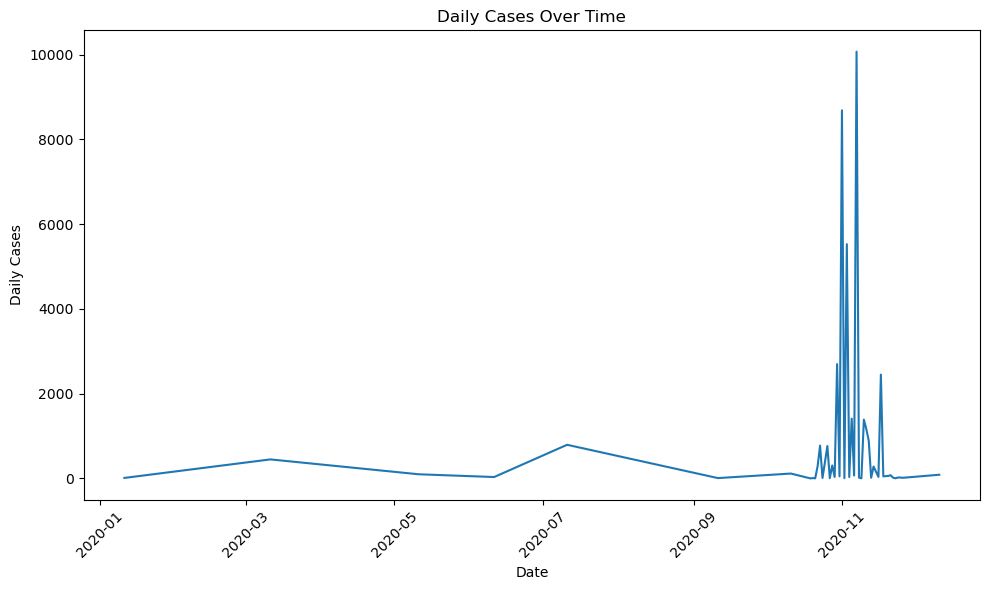
\includegraphics[width=0.9\textwidth]{daily case.png}
\end{frame}

% ACTIVE CASES
\begin{frame}{Active Cases Over Time}
\small
This figure shows the variation in active COVID-19 cases over time.
The trend highlights periods of growth and decline, reflecting changes in transmission dynamics and control measures.
\centering
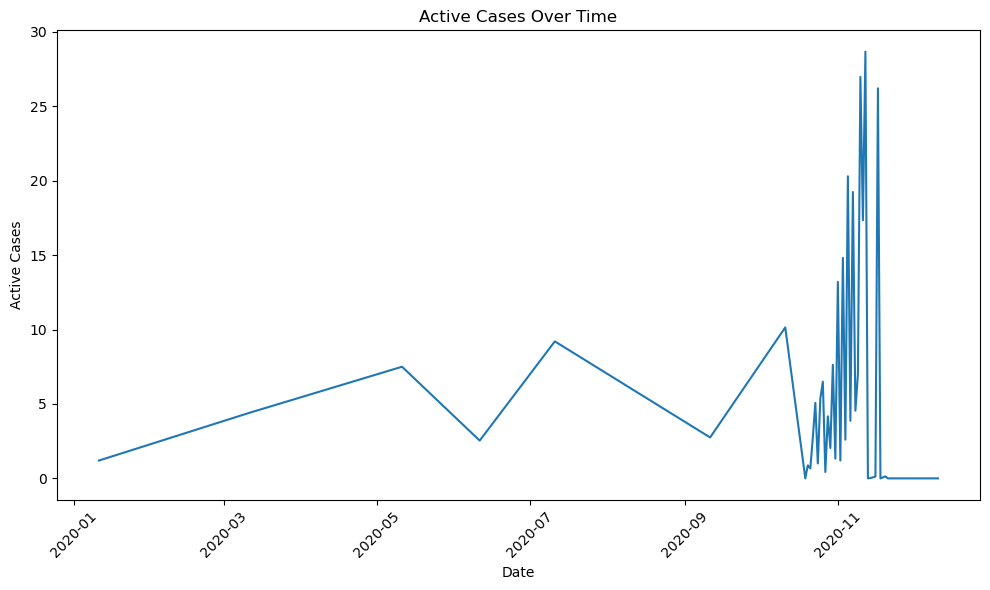
\includegraphics[width=0.9\textwidth]{active case.png}
\end{frame}

% SEIR CURVE
\begin{frame}{Hybrid SEIR Simulation}
\small
The curves illustrate the simulated SEIR dynamics obtained from the hybrid model.
The susceptible population decreases as infections rise, while recovered individuals increase over time.
\centering
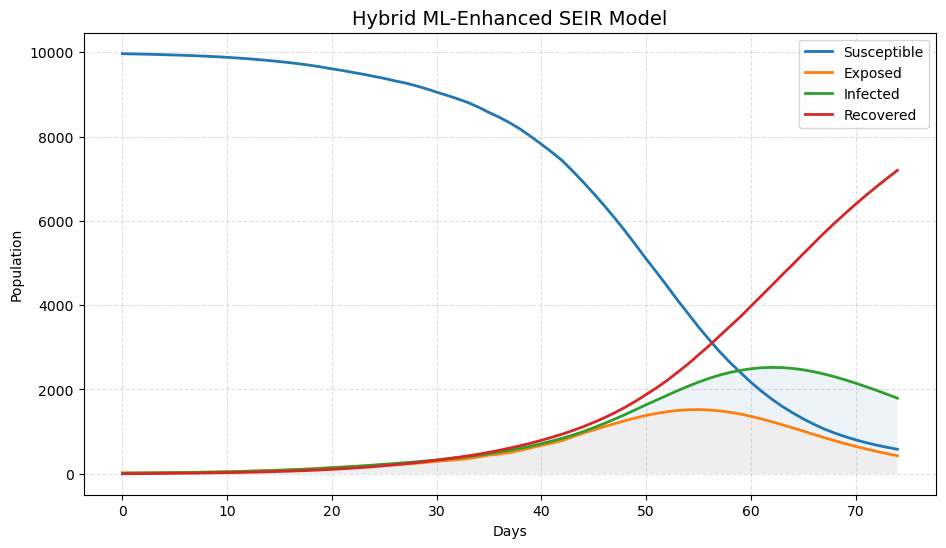
\includegraphics[width=0.9\textwidth]{SEIR model.png}
\end{frame}

% STACKED
\begin{frame}{Top 10 Most vulnerable Area}
\small
The bar chart ranks the top vulnerable regions based on the computed risk score.
Higher values indicate areas requiring priority monitoring and intervention.
\centering
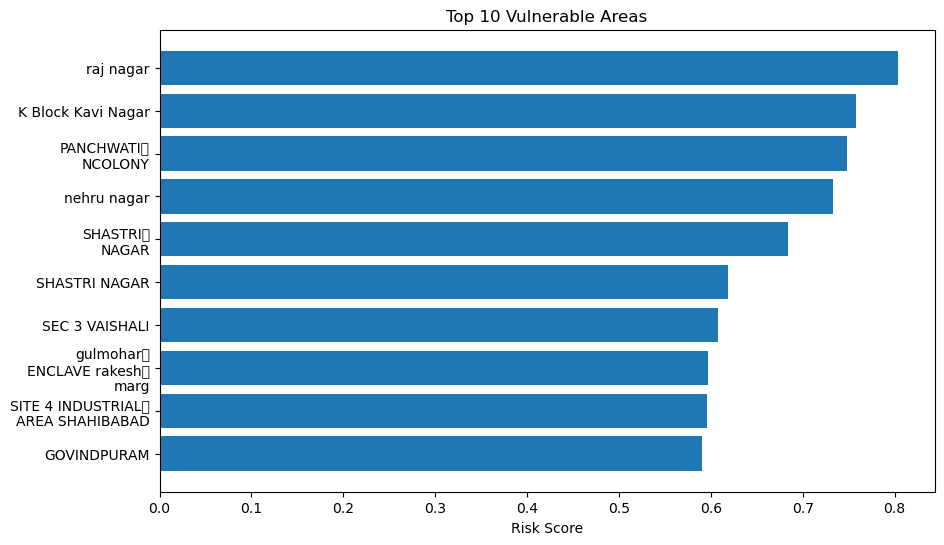
\includegraphics[width=0.9\textwidth]{top 10 area.png}
\end{frame}

% FORECAST
\begin{frame}{Future Infection Prediction}
\small
This figure summarizes the short-term infection forecast for selected regions.
The upward trajectories indicate expected increases, supporting proactive regional planning.
\centering
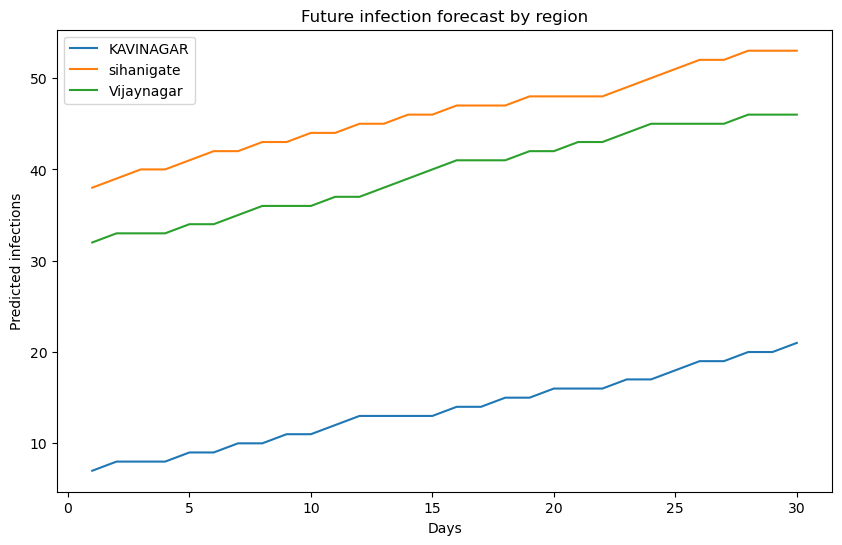
\includegraphics[width=0.9\textwidth]{future predictions.png}
\end{frame}
%--------------------------------
%--------------------------------
\section{Tables}

\begin{frame}{Regional 14-Day COVID-19 Forecast}

The hybrid ML-enhanced SEIR model is used to predict the number of infected individuals
for the next 14 days in the selected region. The table below shows the day-wise forecast.

\begin{table}
\centering
\scriptsize
\resizebox{\textwidth}{!}{
\begin{tabular}{|c|cccccccccccccc|}
\hline
Area & Day1 & Day2 & Day3 & Day4 & Day5 & Day6 & Day7 & Day8 & Day9 & Day10 & Day11 & Day12 & Day13 & Day14 \\
\hline
Kavi Nagar & 19.44 & 28.72	& 42.43	& 62.70	& 92.64	& 136.88 & 202.25 & 298.83 & 441.54 & 652.41 & 963.98 & 1424.34 & 2104.55 & 3109.62
 \\
Rajendra Nagar & 12.22	& 16.73	&22.91	&31.37	&42.95	&58.80	&80.51	&110.24	&150.93	&206.65	&282.94	&387.40	&530.42	&726.24
\\
\vdots & \vdots & \vdots & \vdots & \vdots & \vdots & \vdots & \vdots & \vdots & \vdots & \vdots & \vdots & \vdots & \vdots & \vdots \\
Shashtri Nagar & 11.16	&15.11	&20.44	&27.66	&37.43	&50.66	&68.55	&92.76	&125.52	&169.85	&229.84	&311.02	&420.87	&569.53
\\
\hline
\end{tabular}
}
\caption{Fourteen-day infection forecast generated using the Hybrid SEIR model}
\end{table}

\vspace{0.2cm}
\small
The results indicate a steady rise in predicted infections across regions,
highlighting the usefulness of the hybrid model for short-term regional planning and monitoring.

\end{frame}

%-----------------------------------

\begin{frame}{Area Vulnerability Assessment}

To understand regional risk levels, a vulnerability index is computed
based on population density, healthcare access, and predicted infection growth.

\begin{table}
\centering
\begin{tabular}{|c|c|c|}
\hline
Region & Vulnerability Score & Risk Level \\
\hline
Raj Nagar & 0.80 & High \\
Kavi Nagar & 0.75 & High \\
Nehru Nagar & 0.73 & High \\
Shashtri Nagar & 0.61 & Medium \\
\vdots & \vdots & \vdots \\
Gandhi Nagar & 0.31 & Low \\
\hline
\end{tabular}
\caption{Regional vulnerability classification based on model indicators}
\end{table}

\vspace{0.2cm}
\small
Higher vulnerability scores indicate regions more susceptible to rapid disease spread,
requiring prioritized monitoring and healthcare resource allocation.

\end{frame}

%----------------------------------------

\begin{frame}{SEIR Time Series Evolution}

The SEIR model simulates the temporal evolution of the population
across Susceptible, Exposed, Infectious, and Recovered compartments.

\begin{table}
\centering
\scriptsize
\begin{tabular}{|c|c|c|c|c|}
\hline
Day & $S(t)$ & $E(t)$ & $I(t)$ & $R(t)$ \\
\hline
0 & 9968&19	&13	&0 \\
1&9963&20&15&1 \\
2&9958&21&18&3 \\
3&9952&23&20&5 \\
4&9945&26&23&7 \\
\vdots & \vdots & \vdots & \vdots & \vdots \\
19 & 9300 & 120 & 210 & 370 \\
\hline
\end{tabular}
\caption{Time-series simulation of SEIR compartments}
\end{table}

\vspace{0.2cm}
\small
The results show decreasing susceptible population and increasing recovered individuals,
illustrating the dynamic progression of the epidemic over time.

\end{frame}
%--------------------------------
\begin{frame}{Future Infection Forecast}

\tiny{Using the hybrid ML-enhanced SEIR model, future infection counts are predicted
for different regions over upcoming days. The table below summarizes the expected cases.}

\begin{table}
\centering
\begin{tabular}{|c|c|c|}
\hline
Region & Day & Predicted Infected \\
\hline
Kavi Nagar & 1  & 7 \\
Kavi Nagar & 2  & 8 \\
\vdots & \vdots & \vdots\\
Kavi Nagar & 30 & 21 \\
\hline
Sihani Gate & 1  & 38 \\
Sihani Gate & 2  & 39 \\
\vdots & \vdots & \vdots\\
Sihani Gate & 30 & 53 \\
\hline
\vdots & \vdots & \vdots\\
\hline
Kaushambi & 1  & 105 \\
Kaushambi & 2  & 105 \\
\vdots & \vdots & \vdots\\
Kaushambi & 30 & 155 \\
\hline
\end{tabular}
\caption{Future infection forecast by region and day}
\end{table}

\vspace{0.2cm}
\tiny{The forecast highlights increasing infection trends over time, enabling early
intervention planning and resource allocation for high-risk regions.}

\end{frame}

%--------------------------------
\section{Conclusion}
\begin{frame}{Conclusion}

\begin{itemize}
\item A hybrid machine learning–enhanced SEIR framework was developed to model and forecast regional COVID-19 spread.
\item The integration of data-driven parameter estimation improves prediction accuracy compared to classical SEIR models.
\item Time-series simulations and regional forecasts demonstrate the model’s ability to capture infection trends and population transitions.
\item Vulnerability assessment helps identify high-risk areas for targeted monitoring and healthcare planning.
\item The proposed approach can support short-term epidemic forecasting and informed public health decision-making.
\end{itemize}

\end{frame}

%--------------------------------
\begin{frame}{Future Scope and Aspects}

\textbf{Future Scope}
\begin{itemize}
\item Integrate vaccination dynamics and immunity waning into the SEIR model.
\item Use real-time regional health data for adaptive forecasting.
\item Extend the model to multiple interacting regions to study spatial disease spread.
\end{itemize}

\vspace{0.3cm}

\textbf{Future Aspects}
\begin{itemize}
\item Incorporate mobility patterns, demographic factors, and environmental influences.
\item Explore advanced machine learning approaches such as deep learning or ensemble models.
\item Apply the hybrid SEIR framework to other infectious diseases and epidemic scenarios.
\end{itemize}

\end{frame}
%--------------------------------
\begin{frame}
\centering
\Huge Thank You
\end{frame}

%--------------------------------
\end{document}
